\documentclass{article}
\usepackage{graphicx}
\usepackage[utf8]{inputenc}
\usepackage{listings}
\usepackage{color}
\usepackage{xcolor}
\usepackage{textcomp}
\usepackage{amsmath}
\usepackage{mathabx}

\definecolor{solarized@base03}{HTML}{002B36}
\definecolor{solarized@base02}{HTML}{073642}
\definecolor{solarized@base01}{HTML}{586e75}
\definecolor{solarized@base00}{HTML}{657b83}
\definecolor{solarized@base0}{HTML}{839496}
\definecolor{solarized@base1}{HTML}{93a1a1}
\definecolor{solarized@base2}{HTML}{EEE8D5}
\definecolor{solarized@base3}{HTML}{FDF6E3}
\definecolor{solarized@yellow}{HTML}{B58900}
\definecolor{solarized@orange}{HTML}{CB4B16}
\definecolor{solarized@red}{HTML}{DC322F}
\definecolor{solarized@magenta}{HTML}{D33682}
\definecolor{solarized@violet}{HTML}{6C71C4}
\definecolor{solarized@blue}{HTML}{268BD2}
\definecolor{solarized@cyan}{HTML}{2AA198}
\definecolor{solarized@green}{HTML}{859900}

\lstset{
  language=Java,
  upquote=true,
  columns=fixed,
  tabsize=2,
  extendedchars=true,
  breaklines=true,
  frame=single,
  numbers=left,
  numbersep=5pt,
  rulesepcolor=\color{solarized@base03},
  numberstyle=\tiny\color{solarized@base01},
  basicstyle=\footnotesize\ttfamily,
  keywordstyle=\color{solarized@green},
  stringstyle=\color{solarized@cyan}\ttfamily,
  identifierstyle=\color{solarized@blue},
  commentstyle=\color{solarized@base01},
  emphstyle=\color{solarized@red}
}
\begin{document}

\title{Tarea 2}
\author{Angel Caceres Licona}

\maketitle


\section{1 Haga un análisis de propagación para la resta...}
Tenemos la resta que produce un error definida como 
\begin{equation}
    E= (a \dotdiv b) - (a-b)
\end{equation}
Si además cada uno de estos tiene un error 

\begin{equation}
    \begin{aligned}   
    a^* & = a + \epsilon_a\\
    b^* & = b + \epsilon_b
    \end{aligned}   
\end{equation}

reescribimos la resta como

\begin{equation}
    \begin{aligned} 
    E & = (a^* - b^*) - (a-b)\\
    E & = a + \epsilon_a - b - \epsilon_b - a + b \\
    \epsilon_c &= \epsilon_a -  \epsilon_b
    |\epsilon_c| \leq |\epsilon_a| -  |\epsilon_b|
\end{aligned}   
\end{equation}

\section{2 Elabore un programa que sume el numero 0.0001 10,000 veces consigo mismo...}

\begin{lstlisting}
    public strictfp class Suma {

        public static void main(String[] args) {
        Float numerof = 0.0001
        Double numerod = 0.0001
            for(int i = 1; i < 10000; i++) {
                numerof = numerof + 0.0001
                numerod = numerod + 0.0001
            }
        System.out.println("El resultado de sumar 0.0001 10,000 veces con precision sencilla es " + numerof)
        System.out.println("El resultado de sumar 0.0001 10,000 veces con precision doble es " + numerod)
        }    
            
    }
\end{lstlisting}
La salida del programa es la siguiente: 

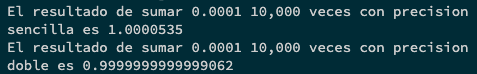
\includegraphics[scale=0.75]{resultadoSumaTarea2.png}
\linebreak 
a) Mi resultado es diferente de 1.
\linebreak 
b) Hice el programa con 0.00001 y 0.000001 y obtuve los siguientes resultados:
\linebreak 
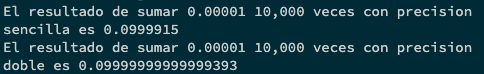
\includegraphics[scale=0.75]{SumaPequenos.png}
\linebreak 
\includegraphics[scale=0.75]{SumaPequenos2.png}
\linebreak 
c) En este caso creo que es posible obtener resultados menores que 1 porque el error que se va acumulando excede la precisión de la variable usada. 
Entonces en cada paso va guardando un numero menor que el que debería obtenerse y ese error se va acumulando.

\section{Evalúe la expresión $\frac{A}{1-\cos x}$ en un valor cercano $x=0$...}
Para esto usaremos la serie de Taylor
\begin{equation}
    f(a^*)-f(a)\approx f'(a)(a^*-a)
\end{equation}
considerando
\begin{equation}
    f'(a)=-\frac{A\sin(x)}{(1-\cos(x))^2}
\end{equation}
y tomaré $a^* = 0.0001$. Sustituyendo obtenemos:
\begin{equation}
    f(0.0001)\approx \frac{1-\sin(0.0001)}{(1-\cos(0.0001))^2}(0.0001-0) - \frac{1}{1-(\cos 0.0001)}
\end{equation}
Para un valor arbitrario de $A$, en este caso 1 obtengo el siguiente valor: $3.9999x10^{12}$ y el valor de $f(0.0001) = 200,000,000$
Yo creo que la aproximación podría mejorarse tomando más términos de la serie de Taylor.

\section{Se desea evaluar la expresión $f(x)=e^{5x}$...}
Tomamos la expresión
\begin{equation}
    |\epsilon_f| \approx |f'(a^*)||\epsilon_a|
\end{equation}
Sustituimos los valores:
\begin{equation}
\begin{aligned}    
    |\epsilon_f| &  \approx  |5e^5{1.01}||0.01| \\
    \epsilon_f & \approx  7.49486
\end{aligned}   
\end{equation}
El resultado de de $e^{1} - e^{1.01}$ es $148.413 - 156.022 = 7.609$ que es similar a lo que predice la expresion anterior.
\section{Codifique el siguiene algoritmo usando precision sencilla...}
Los resultados son los siguientes:
\linebreak
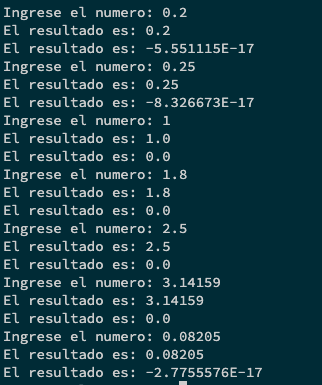
\includegraphics[scale=0.75]{resultadosAlgoritmoSencilla.png}
\linebreak
Lo que veo es que mientras es mas pequeño el numero que estoy evaluando el resultado que incluye la resta es menos preciso.
Al cambiar a precision doble obtengo los siguientes resultados:
\linebreak
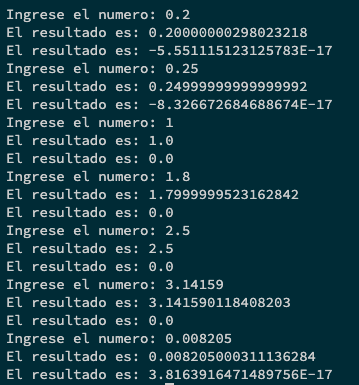
\includegraphics[scale=0.75]{resultadoAlgoritmoPrecisionDoble.png}
\linebreak
En el caso del resultado que incluye la resta del valor original, veo que aunque la primer operación no da el mismo resultado la resta si da cero, lo cual me da a entender que hay un error que rebasa la precision de la variable.

En el caso en el que se está elevando al cuadrado curiosamente si obtuve los resultados esperados para precision sencilla
\linebreak
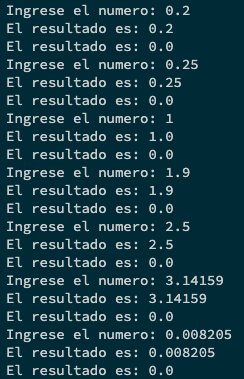
\includegraphics[scale=0.75]{resultadoAlgoritmoCuadradoSencilla.png}
\linebreak
y para precision doble
\linebreak
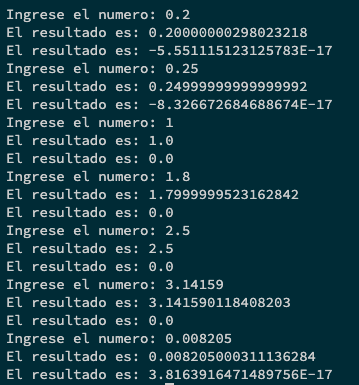
\includegraphics[scale=0.75]{resultadoAlgoritmoPrecisionDoble.png}
\linebreak
El codigo es el siguiente:
\begin{lstlisting}
    public strictfp class algoriitmoTarea2 {

        public static void main(String[] args) {
        Double numero = 0.01
        Double resultado = 0.0
        
        while(numero > 0){
            print "\nIngrese el numero: "
            numero = System.in.newReader().readLine() as Double
            if(numero < 0){
                break
            }
            resultado =  Math.sqrt(Math.pow(numero,2))
            print "El resultado es: " + resultado
            resultado = Math.sqrt(Math.pow(numero,2)) - numero
            print "\nEl resultado es: " + resultado
        }
        
        }    
            
    }
\end{lstlisting}
\end{document}